%--------------------------------------------------------------------------------------------------
\section{Image Recognition Models}
\label{rel:sec_imrecon}
Image recognition is a subtask of computer science that aims at replicating human vision 
capabilities with a machine. From its early developments  with David Marr's postulates 
on vision (\cite{poggio1981marr}, \cite{marr2010vision}), this field has been approached on a 
computational level since the 1980s. Following this, early works in computer vision 
paved the way for the application of classical machine learning models on image recognition. In 
the beginning, researchers focused on fundamental challenges such as edge detection and image 
segmentation. The 1970s and 1980s witnessed pioneering efforts, with 
techniques like the Hough Transform for line detection and the development of feature-based 
methods \autocite{duda1972use}. These early approaches set the groundwork for the later integration 
of classical machine learning models, as they provided preliminary insight into how visual 
information could be analyzed and processed computationally. The emergence of classical machine 
learning models, and their application in the 1980s, marked a shift towards more sophisticated 
image recognition methodologies.\\

%--------------------------------------------------------------------------------------------------
\subsection{Traditional Image Recognition models}
\noindent Traditional image recognition approaches based on traditional machine learning 
algorithms are a two-step process. The first step involves the extraction of features from the 
data, and the last step lies in the training of a classifier. Examples of this 
can be found in methodologies such as \gls{sift} \autocite{lowe1999object}, \gls{bow} 
\autocite{csurka2004visual}, and \gls{hog}. 
SIFT, stands out as a powerful keypoint detector that incorporates image alignment. 
More importantly, its robustness towards scale and rotation led to widespread adoption in real 
world applications \autocite{cruz2012scale}.
Complementary to SIFT and adopting ideas based on \gls{nlp}, the concept behind the BOW descriptor 
originated from the identification of keywords on a text, in order to identify its contents 
\autocite{harris1954distributional}. On itself BOW extracts features akin to SIFT, clustering them 
to generate a dictionary which will ultimately form the possible words to describe images. Each 
image is recognized by the frequency of which certain words are used to describe it.
Finally, HOG follows a simpler approach, where image gradient information is organized in histograms 
describing the orientation of image components. \\ 

%--------------------------------------------------------------------------------------------------
\noindent Once image descriptors are extracted, classifiers are trained using algorithms such as 
\gls{svm} \autocite{cortes1995support}, Random Forests \autocite{ho1995random} and \gls{knn}
(\cite{cover1967nearest}, \cite{fix1989discriminatory}). \glspl{svm} are classifiers that operate 
by finding the most optimal hyperplane in the feature space to discriminate between classes. 
However, challenges arise when the assumption of data being linearly separable is not met. This 
difficulty was addressed with the introduction of the kernel trick \autocite{hofmann2008kernel}, 
where data is transformed to another space where this is more straightforward.\\
Complementary to SVMs, Random Forest Trees is a methodology that constructs a plethora of decision 
trees, where each tree uses a random subset of the training data, and each node uses a random 
subset of features to make a decision. This randomness ensures diversity among trees, providing a 
degree of robustness towards overfitting. On a much simpler note, \gls{knn} operates based on the 
assumption of data being contained in $k$ different categories. The classification method involves 
assigning one category to a data point that is the closest in feature space to a class centroid, 
obtained through K-Means \autocite{macqueen1967some}.\\

%--------------------------------------------------------------------------------------------------
\noindent Although many of the early image recognition models were based on traditional machine 
and statistic methods, neuroscience research still inspired scholars to propose alternative 
approaches. Moreover, with studies on the visual cortex regarding receptive fields 
\autocite{hubel1959receptive}, the development of \glspl{nn} started. Notably, the 
Neocognitron \autocite{fukushima1975cognitron} sparked the inception of  Ns, introducing 
kernel operations, hierarchical feature aggregation and non-linearities. These contributions stand 
out as they are key components in most recent image recognition models.
Still, the hierarchical properties and aggregation of the Neocognitron did not really achieve 
a great deal of momentum on early days; around this time, other image recognition models were being 
used yielding better results, examples of this can be seen with the amount of traditional machine 
learning based methods that dominated this task around that time. Nevertheless, getting close to the 
dawn of the year 2000, Yann LeCun proposed LeNet to perform digit recognition 
\autocite{lecun1998gradient} the first modern \gls{cnn}.\\

%--------------------------------------------------------------------------------------------------
\subsection{Convolutional Neural Networks}
\label{rel:sub_cnn}
Starting with LeNet, the convolution took prominence as the fundamental building block 
of most current image recognition models. In the domain of computer vision, the convolution is an 
interaction ($f\star g$) between a feature map ($f$), and a kernel ($g$), as shown in  
\autoref{fig:conv_local}. In particular, the convolutional kernel $g$ is mediated by its area 
determined by width and height, influencing directly its receptive field. The 
receptive field answers to the area within the input space covered by the convolutional kernel. 
Furthermore, during convolution, the kernel slides over the feature map, computing the dot product 
between the kernel $g$, over the area it covers in the input map centered around each pixel. 
Consequently, in deep layers of a \gls{cnn} this computation encompasses larger regions of the 
input image, allowing the model to capture long range dependencies and enhance its capabilities. 
Additionally, convolutions present similarities to SIFT, such as their ability to construct 
representations invariant to image alterations, and utilize receptive fields for feature extraction.

%--------------------------------------------------------------------------------------------------
\begin{figure}[h]
    \centering
    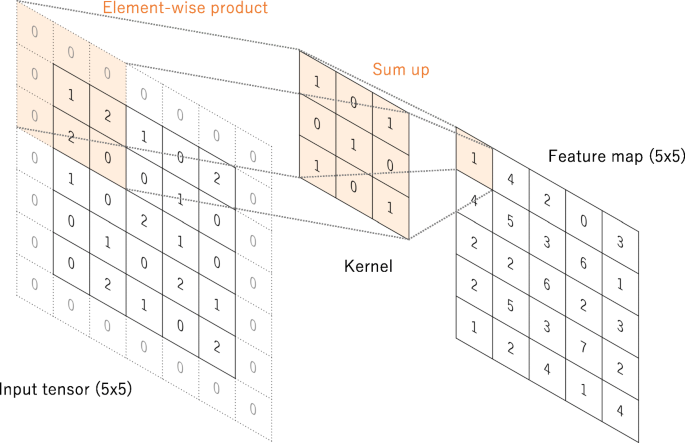
\includegraphics[width=\textwidth]{fig/rel/images/conv_not_proper.png}
    \caption{Illustration of the convolution operation. Properties, parameters and behaviour.}
    \label{fig:conv_local}
\end{figure}
%--------------------------------------------------------------------------------------------------
\noindent On top of convolutions, LeNet led to the introduction of more components of \glspl{cnn}: 
pooling operations and non-linearities. Pooling operations are used to reduce the spatial 
resolution of feature maps, which in turn aids convolutions in capturing features from long 
range dependencies within the image. Moreover, via pooling it is possible to capture the most 
relevant features within a neighborhood.
Conversely, non-linearities such as Sigmoid and ReLU \autocite{fukushima1969visual}, are designed to 
capture complex relationships within data, stopping the model collapsing into a linear operation. 
Furthermore, these operations also contribute with stability: they maintain values within feature 
maps and the gradient in ranges in which the network can operate with. Additionally, it is possible 
to control the flow of information within the network with operations such as Dropout. This 
operation randomly deactivates units on a convolutional layer, forcing the model to learn more 
robust representations as it cannot rely on a set of previously learned features consistently. %cite this?
Still, the key contribution leading to the success of LeNet was not only the usage of 
convolutions, pooling and non-linearities; but its training process, that guided by gradient descent 
to optimize, ultimately enabled \glspl{cnn} to outperform traditional computer vision methods for 
document recognition. \\

%--------------------------------------------------------------------------------------------------
\noindent With the advent of the 2010s and the initiation of the \gls{ilsvrc} \autocite{ILSVRC15} 
a proper environment for further development of models was established. Unlike prior datasets, 
ImageNet was composed of images that presented more complexity than earlier datasets. Instead 
of catalog-like compositions; elements in this dataset closely resemble those found 
in the wild, featuring multiple classes or instances of a class within a single image.\\

%--------------------------------------------------------------------------------------------------
\noindent Upon its release, several traditional approaches were trained and evaluated on this 
collection, achieving a low performance. However, \glspl{cnn} regained prominence with the 
introduction of AlexNet \autocite{krizhevsky2012imagenet}. Inspired by LeNet, Krizhevsky designed a 
\gls{cnn} that incorporated additional convolutions and, more importantly, facilitated faster 
computation through effective communication with the \gls{gpu}.
AlexNet gained notoriety by emerging as the winner of the 2012 \gls{ilsvrc}, achieving a top-1 
classification accuracy difference of nearly 10\% compared to previous year winners 
(\cite{berg2010large}, \cite{sanchez2011high}). This substantial improvement in recognition 
capabilities led to a paradigm shift in various machine learning tasks, laying the foundation 
for the deep learning revolution.
Following this success, several \glspl{cnn} were introduced in the decade of 2010, and since then;
a considerable amount of models have been proposed. Nevertheless, we can establish a timeline with the 
milestone models that influenced the most this development, as seen in \autoref{fig:cnn_timeline}
and iterate upon the performance of some of these models in \autoref{tab:rel_recon}.\\

%--------------------------------------------------------------------------------------------------
\begin{figure}[H]
    \centering
    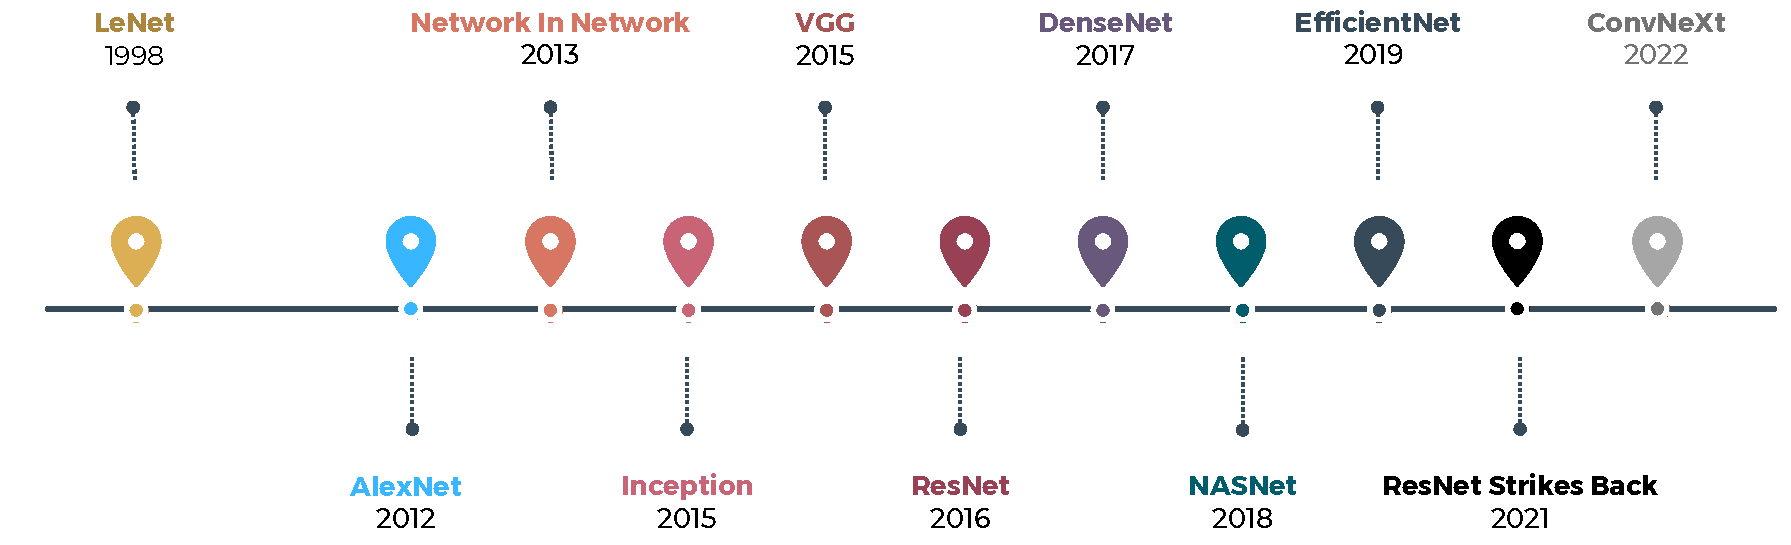
\includegraphics[width=\textwidth]{fig/rel/images/CNN_timeline.pdf}
    \caption{\textbf{Timeline} of milestone Deep Learning models.}
    \label{fig:cnn_timeline}
\end{figure}
\begin{table}[H]
    \centering
    \footnotesize
    \begin{tabular}{lcccccc}\toprule
        \Th{Method} & \Th{Release Year} & \Th{Acc@1} & \Th{Acc@5} & \Th{Params} & \Th{GFLOPS}\\\midrule
        AlexNet&2012&51.52&79.07&61.1M&0.71\\
        VGG-16&2015&73.36&91.52&138.4M&15.47\\
        ResNet50&2016&76.13&92.86&25.6M&4.09\\
        EfficientNet-B0&2019&77.69&95.32&5.3M&0.38\\
        ViT-Base&2020&81.07&95.32&86.6M&17.56\\
        ResNet-50*&2021&80.86&95.43&25.6M&4.09\\
        ConvNeXt-Base&2022&84.06&96.87&88.6M&15.36\\\bottomrule
    \end{tabular}
    \caption{\textbf{Milestone Image Recognition Methods} Details of milestone Image recognition models in the era of Deep Learning on ImageNet 1k. 
    ResNet* refers to the version using updated training protocols \autocite{wightman2021resnet}}%}
\label{tab:rel_recon}
\end{table}
%--------------------------------------------------------------------------------------------------
\noindent In the year following the publication of AlexNet, an updated form of mapping feature maps 
into classification embeddings was proposed  in the shape of \gls{gap} \autocite{lin2013network}. 
This pooling protocol generates a representation taking the average value of each feature map 
channel, as shown in \autoref{fig:rel_gap}. Furthermore, \gap reduces dimensionality and regularizes 
the model using global aggregation; in turn improving classification performance.\\ 
\begin{figure}[H]
    \centering
    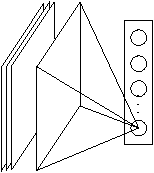
\includegraphics[width=0.15\textwidth]{fig/rel/images/gap_fix.pdf}
    \caption{Visual representation of Global Average Pooling \autocite{lin2013network}.}
    \label{fig:rel_gap}
\end{figure}

%--------------------------------------------------------------------------------------------------
\noindent Similar to 2012 and 2013, 2015 saw the proposal of two milestone models: the Inception 
architecture \autocite{szegedy2015going} and VGG models \autocite{simonyan2015deep}. On one hand, 
the Inception architecture was designed to learn features in different scale. To achieve this, the 
\emph{Inception Block} introduced the \emph{Inception Block}, which captures multiscale behavior 
by incorporation  of convolutional kernels with sizes of $5\times5$, $3\times 3$ 
and $1\times1$. On the other hand, VGG models were built with a simplistic design, relying solely 
on $3\times 3$ convolutions. For a change, VGG is shown to be an excellent feature extractor 
network. Led by the desire to increase depth of \glspl{cnn}, VGG and Inception attempted to make 
models deeper; nevertheless this was not possible. As models get deeper, the gradient becomes zero 
when flowing from deep layers to shallow layers, denying updates to their 
parameters. This is known as the vanishing gradient issue \autocite{pascanu2013difficulty}. To address this issue, the ResNet architecture was 
proposed \autocite{he2016deep}.\\

%--------------------------------------------------------------------------------------------------
\begin{figure}[t]
    \centering
    \scriptsize
    \begin{tabular}{cc}
        \mc{2}{\begin{tikzpicture}[
        font={\footnotesize},
        trap/.style={trapezium, rotate=-90,trapezium angle=75},
    ]
        %% CNN branch
        \node(input) at (0, 0) {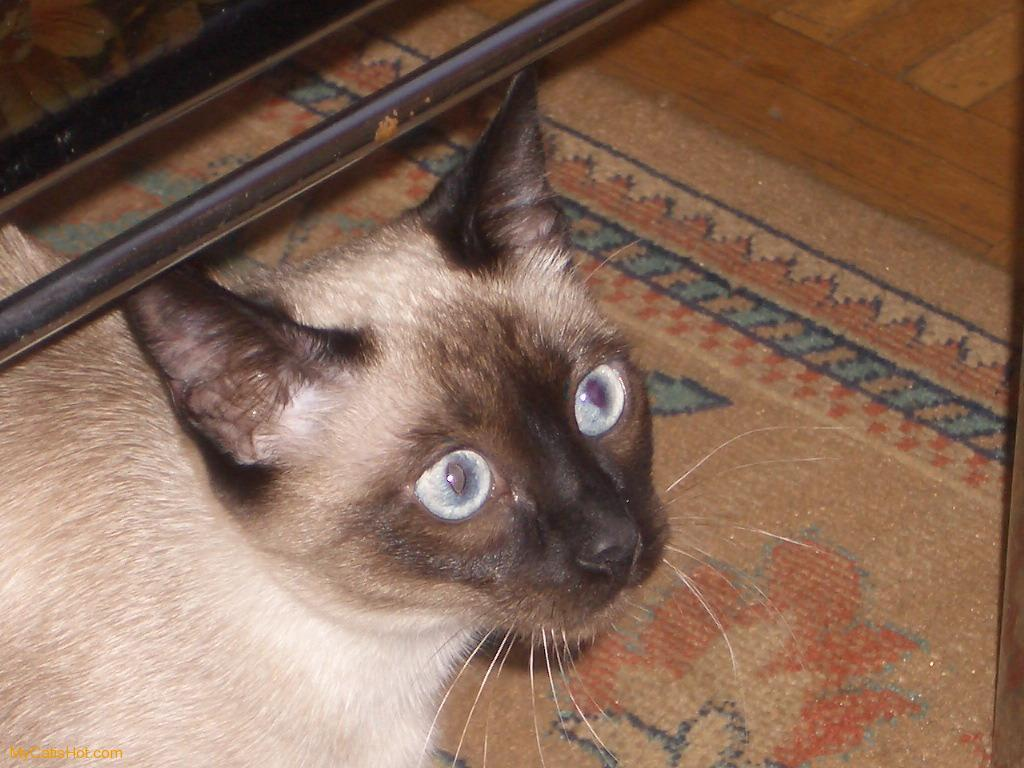
\includegraphics[width=.1\textwidth]{fig/castream/images/input.jpg}};
        \node[above] at (input.north) {Input image};
        \node[draw, rotate=90, align=center](conv1) at (2, 0) {\Th{conv} $7\times7$};
        %\node[draw, rotate=90, align=center](bn) at (-3, 0) {\Th{BatchNorm}};
        %\node[draw, rotate=90, align=center](relu) at (-2.5, 0) {\Th{ReLU}};
        %\node[draw, rotate=90, align=center](maxp) at (-2, 0) {\Th{MaxPool}};
        \node[draw, trap] (res1) at (4,0) {\rotatebox{90}{\parbox{1.0cm}{\centering{\Th{Res-1}}}}};
        \node[draw, trap] (res2) at (6,0) {\rotatebox{90}{\parbox{1.0cm}{\centering{\Th{Res-2}}}}};
        \node[draw, trap] (res3) at (8,0) {\rotatebox{90}{\parbox{1.0cm}{\centering{\Th{Res-3}}}}};
        \node[draw, trap] (res4) at (10,0) {\rotatebox{90}{\parbox{1.0cm}{\centering{\Th{Res-4}}}}};
        %\node[](empt1) at (6.25, 0){};
        \node[draw, rotate=90, align=center] (class) at (12,0) {Classifier};
        \node(logit) at (13, 0) {$\vy$};
    
        %% CNN backbone
        %\node(empt0) at (-4.65, 0) {};
        \draw[->] (input.east) -- node {} (conv1);
        \draw[->] (conv1.south) -- node[above] {$F_0$} (res1);
        %\draw[->] (empt0.center) -- node {} (conv1);
        \draw[->] (res1) -- node[above] {$F_1$} (res2);
        \draw[->] (res2) -- node[above] {$F_2$} (res3);
        \draw[->] (res3) -- node[above] {$F_3$} (res4);
        \draw[->] (res4) -- node [above] {} (class);
        \node[](GAP) at (11.125,0.25) {\gls{gap}};
        \draw[->] (class) -- node {} (logit);
\end{tikzpicture}
    }\\
        \mc{2}{$a.$ ResNet Architecture}\\
        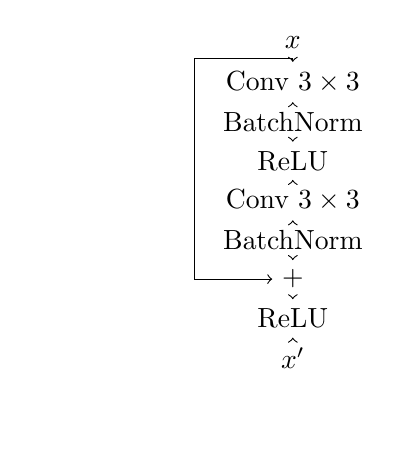
\begin{tikzpicture}[]
    % Nodes
    \node at (1.75,0) (input){$x$};
    \node[align=center] (conv1) at (1.75, -.5) {\Th{Conv} $3\times3$};
    \node[align=center] (bn1) at (1.75, -1) {\Th{BatchNorm}};
    \node[align=center] (relu1) at (1.75, -1.5) {\Th{ReLU}};
    \node[align=center] (conv2) at (1.75, -2) {\Th{Conv} $3\times3$};
    \node[align=center] (bn2) at (1.75, -2.5) {\Th{BatchNorm}};
    \node[align=center] (sum) at (1.75, -3) {$+$};
    \node[align=center] (relu2) at (1.75, -3.5) {\Th{ReLU}};
    \node(output) at (1.75, -4) {$x'$};
    \node at (1.75,-0.2) (empt0) {};
    \node at (0.5, -2) (empt1) {};
    \node at (-1.5, 0) (emptkek) {};

    \node at (0, -5) (emptbal) {};
    

    %% CNN Edges
    \draw[->] (input.south) -- node {} (conv1);
    \draw[->] (conv1.south) -- node  {} (bn1.north);
    \draw[->] (bn1.south) -- node  {} (relu1.north);
    \draw[->] (relu1.south) -- node  {} (conv2.north);
    \draw[->] (conv2.south) -- node  {} (bn2.north);
    \draw[->] (bn2.south) -- node  {} (sum.north); 
    \draw[-] (empt0.center) -| node {} (empt1.center);
    \draw[->] (empt1.center) |- node {} (sum.west);
    \draw[->] (sum.south) -- node  {} (relu2.north);
    \draw[->] (relu2.south) -- node  {} (output.north);
\end{tikzpicture}
&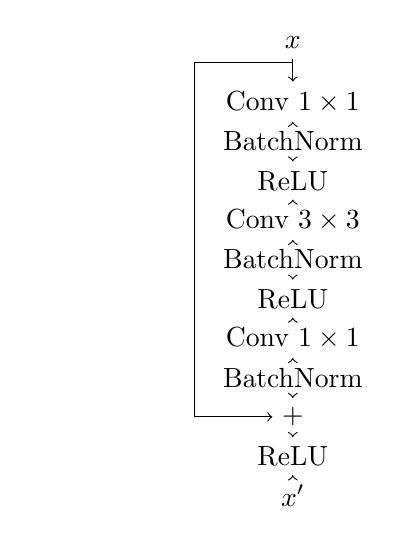
\begin{tikzpicture}[]
    % Nodes
    \node at (1.75,0.25) (input){$x$};
    \node[align=center] (conv1) at (1.75, -0.5) {\Th{Conv} $1\times1$};
    \node[align=center] (bn1) at (1.75, -1) {\Th{BatchNorm}};
    \node[align=center] (relu1) at (1.75, -1.5) {\Th{ReLU}};

    \node[align=center] (conv2) at (1.75, -2) {\Th{Conv} $3\times3$};
    \node[align=center] (bn2) at (1.75, -2.5) {\Th{BatchNorm}};
    \node[align=center] (relu2) at (1.75, -3.0) {\Th{ReLU}};

    \node[align=center] (conv3) at (1.75, -3.5) {\Th{Conv} $1\times1$};
    \node[align=center] (bn3) at (1.75, -4) {\Th{BatchNorm}};
    \node[align=center] (sum) at (1.75, -4.5) {$+$};

    \node[align=center] (relu3) at (1.75, -5) {\Th{ReLU}};
    \node(output) at (1.75, -5.5) {$x'$};
    \node at (1.75,-0) (empt0) {};
    \node at (0.5, -2.75) (empt1) {};
    \node at (-1.5, 0) (emptkek) {};
    

    %% CNN Edges
    \draw[->] (input.south) -- node {} (conv1);
    \draw[->] (conv1.south) -- node  {} (bn1.north);
    \draw[->] (bn1.south) -- node  {} (relu1.north);
    \draw[->] (relu1.south) -- node  {} (conv2.north);

    \draw[->] (conv2.south) -- node  {} (bn2.north);
    \draw[->] (bn2.south) -- node  {} (relu2.north); 
    \draw[->] (relu2.south) -- node  {} (conv3.north);

    \draw[->] (conv3.south) -- node  {} (bn3.north);
    \draw[->] (bn3.south) -- node  {} (sum.north); 
    \draw[-] (empt0.center) -| node {} (empt1.center);
    \draw[->] (empt1.center) |- node {} (sum.west);
    \draw[->] (sum.south) -- node  {} (relu3.north);
    \draw[->] (relu3.south) -- node  {} (output.north);
\end{tikzpicture}
\\
        $b.$ Basic Block Residual Block & $c.$ Bottleneck Residual Block \\
    \end{tabular}
    \caption{Generalities of the ResNet architecture. Overall architecture and Residual Block Design.}   
    \label{fig:resnet}
\end{figure}
%--------------------------------------------------------------------------------------------------
%\begin{tikzpicture}[
        font={\footnotesize},
        trap/.style={trapezium, rotate=-90,trapezium angle=75},
    ]
        %% CNN branch
        \node(input) at (0, 0) {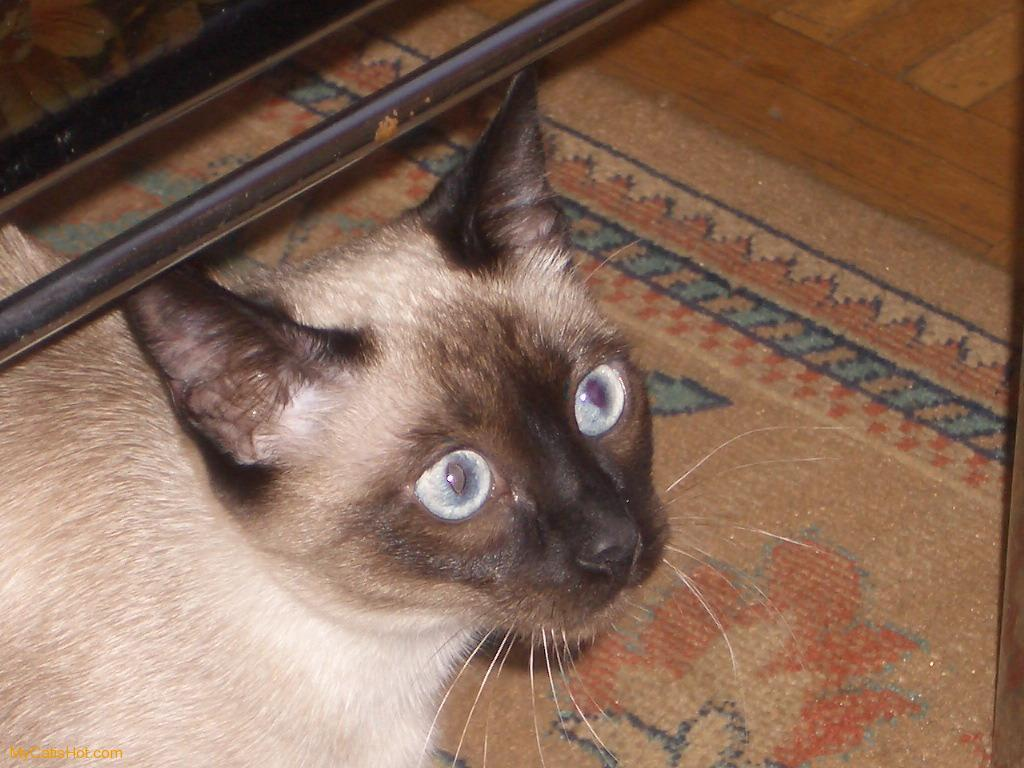
\includegraphics[width=.1\textwidth]{fig/castream/images/input.jpg}};
        \node[above] at (input.north) {Input image};
        \node[draw, rotate=90, align=center](conv1) at (2, 0) {\Th{conv} $7\times7$};
        %\node[draw, rotate=90, align=center](bn) at (-3, 0) {\Th{BatchNorm}};
        %\node[draw, rotate=90, align=center](relu) at (-2.5, 0) {\Th{ReLU}};
        %\node[draw, rotate=90, align=center](maxp) at (-2, 0) {\Th{MaxPool}};
        \node[draw, trap] (res1) at (4,0) {\rotatebox{90}{\parbox{1.0cm}{\centering{\Th{Res-1}}}}};
        \node[draw, trap] (res2) at (6,0) {\rotatebox{90}{\parbox{1.0cm}{\centering{\Th{Res-2}}}}};
        \node[draw, trap] (res3) at (8,0) {\rotatebox{90}{\parbox{1.0cm}{\centering{\Th{Res-3}}}}};
        \node[draw, trap] (res4) at (10,0) {\rotatebox{90}{\parbox{1.0cm}{\centering{\Th{Res-4}}}}};
        %\node[](empt1) at (6.25, 0){};
        \node[draw, rotate=90, align=center] (class) at (12,0) {Classifier};
        \node(logit) at (13, 0) {$\vy$};
    
        %% CNN backbone
        %\node(empt0) at (-4.65, 0) {};
        \draw[->] (input.east) -- node {} (conv1);
        \draw[->] (conv1.south) -- node[above] {$F_0$} (res1);
        %\draw[->] (empt0.center) -- node {} (conv1);
        \draw[->] (res1) -- node[above] {$F_1$} (res2);
        \draw[->] (res2) -- node[above] {$F_2$} (res3);
        \draw[->] (res3) -- node[above] {$F_3$} (res4);
        \draw[->] (res4) -- node [above] {} (class);
        \node[](GAP) at (11.125,0.25) {\gls{gap}};
        \draw[->] (class) -- node {} (logit);
\end{tikzpicture}
    
\noindent The ResNet architecture is designed with the idea of residual connections as its 
building block. On itself, a residual block generates outputs via the summation of its input and a 
linear mapping of it. In detail, a residual block takes a feature map and projects it to 
different dimensions, regularizes it through a bottleneck or with activations, and then sums this 
representation with the original input. This in turn enhances the network capabilities to scale in 
size, leading to improvements in performance while being easier to optimize. This architecture 
maintains its relevancy because of its modularity and the aforementioned scaling properties. For 
instance, some of the most important \gls{cnn} based object detectors are designed using ResNet as 
backbone (\cite{ren2015faster}, \cite{lin2017focal}, \cite{he2017mask}). A thorough representation 
of this architecture, as well as the residual connection variants is presented in 
\autoref{fig:resnet}.\\

%--------------------------------------------------------------------------------------------------
\noindent Similarly to the residual connections introduced in ResNet, DenseNet 
\autocite{huang2017densely} was proposed with the idea of connecting all layers operating within 
matching feature-map sizes. We illustrate this on \autoref{fig:dense_schema}. In particular, this 
architecture enables the training of very deep models, as these connections facilitate feature reuse 
and identity mappings, thus negating the effect of vanishing gradients. However, one issue of 
DenseNet is its lack of  modularity and ease of use. Due to a great number of 
neurons being interconnected by design, introducing of modifications such as \gls{nlb} 
\autocite{wang2018non} or Squeeze Excitation Blocks  \autocite{hu2018squeeze} is challenging. In 
contrast, in architectures such as ResNet this procedure is simple.\\

%--------------------------------------------------------------------------------------------------
\begin{figure}[H]
    \centering
    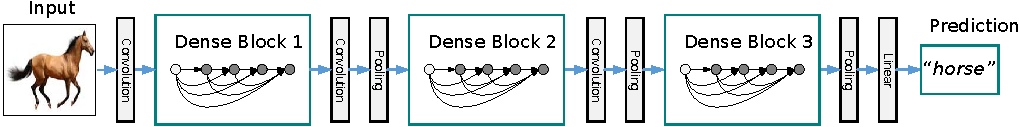
\includegraphics[width=\textwidth]{fig/rel/images/densenet_schema.pdf}
    \caption{\textbf{Illustration of the DenseNet architecture} \autocite{huang2017densely}}
    \label{fig:dense_schema}
\end{figure}
%--------------------------------------------------------------------------------------------------
\noindent Moreover, it is arguable that convolutional block design can be improved if a model 
learns on itself the best configuration possible for a specific task. This is idea is embodied by 
the \gls{nasnet} \autocite{zoph2018learning} where the model learns a fundamental building block on a 
small dataset, and it is then transferred into a larger one. Some of the biggest drawbacks for this 
model, are its computational load and the dependency on search space selection towards 
optimization. One last milestone attempt at improved architecture design was proposed in 2019 with 
EfficientNet \autocite{tan2019efficientnet}. In sharp contrast to its contemporaries approaches at 
scaling; EfficientNet proposes a \emph{compound coefficient} instead.\\

%--------------------------------------------------------------------------------------------------
\noindent Still, some of the aforementioned architectures were not proposed with such 
contributions, and as such it is possible to suggest that an unfair comparison is performed, 
as well as an incomplete study on said model capabilities. One such answer to this issue was 
proposed for ResNet in 2021 \autocite{wightman2021resnet}. In this approach, ResNet was retrained 
under updated training regimes, achieving a high classification performance, rivaling that of 
transformers.\\
%--------------------------------------------------------------------------------------------------
%Alongside these models, several improvements have been introduced to aid the optimization 
%process. In particular, some of the earliest approaches were trained using \gls{sgd} 
%\autocite{bottou2010large}; while Adam \autocite{kingma2014adam} and Lamb \autocite{you2019large} 
%optimizers have taken prominence in later years. Additionally, data augmentation strategies have 
%evolved too; researchers have proposed methodologies to enhance data variability by the 
%incorporation of characteristics of different classes in a particular one within an image 
%(\cite{zhang2017mixup}, \cite{yun2019cutmix}). 
%--------------------------------------------------------------------------------------------------
\noindent Finally, with the advent of transformer based image recognition models in the early years of the 
2020 decade, \glspl{cnn} started being outshone by these models; however, an architecture 
incorporating the key principles of these models was presented, ConvNeXt \autocite{liu2022convnet}.
This family of models addressed some shortcomings of transformer models (mentioned in 
\autoref{rel:sub_att}) and proposed their mitigation with the modernization of a ResNet 
architecture, enhancing its performance not only in image recognition, but also in segmentation and 
detection. Still, having mentioned transformers, we dedicate the following subsection to their 
description, their basic unit and some milestone models.
%% ------------------------------------------------------------------------------------------------
\subsection{Self-Attention Based Architectures}
\label{rel:sub_att}
One key point to remember is that Computer Vision is not isolated within Artificial 
Intelligence; advancements in this field have, conversely, contributed to complementary domains, 
such as \gls{nlp}. Furthermore, proposals made for that domain have found applications into image 
recognition; one such development is that of Transformers. The Transformer architecture was 
initially proposed in 2017 with the article \emph{Attention is All You Need} 
\autocite{vaswani2017attention}. This model addressed limitations in existing methodologies for 
NLP such as LSTMs and RNNs, particularly their struggles in capturing long range dependencies 
and efficient training.\\

%--------------------------------------------------------------------------------------------------
\noindent Similarly to the impact AlexNet had on image recognition, transformers 
revolutionized the landscape of NLP with their key component: \emph{Self-Attention}. This function 
assigns weights to different input sequences, enabling focus on relevant information. 
This is defined in the following manner:
\begin{equation}
    \mbox{Attention}(Q, K, V) = \mbox{softmax}\left(\frac{QK^T}{\sqrt{d_k}}\right) V
    \label{eq:att}
\end{equation}
\noindent where $Q, K, V$ are embedding matrices that represent \emph{queries}, \emph{keys} and 
\emph{values}, each with a dimension $d_k$. The softmax activation function is employed to 
emphasize relevant information for each product between $Q$ and $V$. Conversely, the scaling 
coefficient $\sqrt{d_k}$ uses the square root to prevent softmax from entering regions with small 
gradients, particularly important as large values of $d_k$ produce this outcome. Conversely, for 
each token \emph{self-attention} is then defined as an average of all values (rows of $V$), weighted 
by the attention (corresponding row of A).
\begin{equation}
	\sa(X_\ell) \defn A V \in \real^{t_\ell \times d_\ell}.
\label{eq:SA}
\end{equation}
This function can be further parallelized by broadcasting these embeddings into different 
heads, where the dot products are ultimately easier to compute; this in turn is called \gls{mhsa}.
%--------------------------------------------------------------------------------------------------
Self attention has no parameters whatsoever: this function is utilized in blocks that ultimately 
form the encoder part of the transformer. One encoder block comprises a residual operation where 
the input embedding is updated with the product of \gls{mhsa}, normalized, and then this 
representation is further recombined with the residual operation atop of 
a feed forward network. This is best explained in \autoref{fig:transf_block}.\\

%--------------------------------------------------------------------------------------------------
%--------------------------------------------------------------------------------------------------
\begin{figure}[t]
    \centering
    \begin{tabular}{cc}
        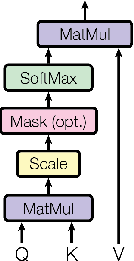
\includegraphics[width=.15\textwidth]{fig/rel/images/scaled_dotproduct.pdf}&
        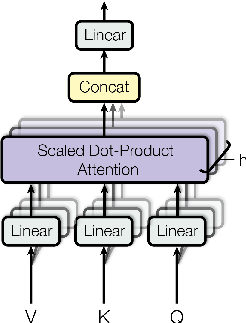
\includegraphics[width=.25\textwidth]{fig/rel/images/mhsa.pdf}\\
        $a.$ Scaled Dot Product Attention & $b.$ Multi Head Self Attention. \\
        & \\
        & \\
        \mc{2}{\small 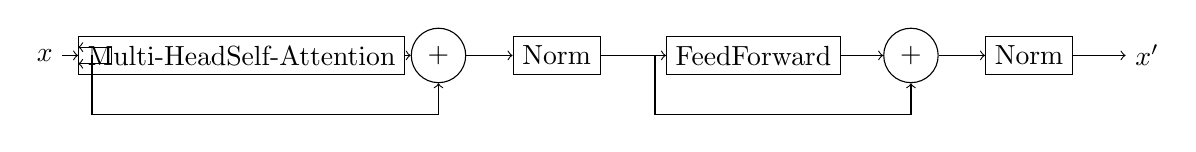
\begin{tikzpicture}[]
        %% Nodes
        \node[rectangle, draw] (mhsa) at (2.5,0)  {Multi-Head\\Self-Attention};
        \node[circle, draw] (sum1) at (5, 0) {$+$};
        \node[rectangle, draw] (norm1) at (6.5,0) {Norm};
        
        \node[rectangle, draw] (ffwd) at (9,0) {Feed\\Forward};
        \node[circle, draw] (sum2) at (11,0) {$+$};
        \node[rectangle, draw] (norm2) at (12.5,0){Norm};

        \node(input) at (0, 0) {$x$};
        \node(output) at (14, 0) {$x'$};
        \node(emptres) at (0.6, 0) {};
        \node(emptres2) at (7.75, 0) {};
        \node(empt0) at (0.85, 0) {};
        \node(empt1) at (2.75, -.75) {};
        \node(empt2) at (10, -.75) {};
        
        
        %% Edges
        \draw[->] (input.east) -- node {} (mhsa.west);
        \draw[->] (empt0.center) |- node {} ([yshift=-4pt] mhsa.north west);
        \draw[->] (empt0.center) |- node {} ([yshift= 4pt] mhsa.south west);
        \draw[-] (emptres.center) |- node {} (empt1.center);
        \draw[->] (empt1.center) -| node {} (sum1.south);
        \draw[->] (mhsa.east) -- node {} (sum1.west);
        \draw[->] (sum1.east) -- node {} (norm1.west);

        \draw[->] (norm1.east) -- node {} (ffwd.west);
        \draw[-] (norm1.east) -- node {} (emptres2.center);
        \draw[-] (emptres2.center) |- node {} (empt2.center);
        \draw[->] (empt2.center) -| node {} (sum2.south);
        \draw[->] (ffwd.east) -- node {} (sum2.west);
        \draw[->] (sum2.east) -- node {} (norm2.west);
        \draw[->] (norm2.east) -- node {} (output.west);
\end{tikzpicture}    }\\
        \mc{2}{$c.$ Transformer encoder block.}\\
    \end{tabular}
    \caption{\textbf{Transformer} self attention variants and encoder block.}
    \label{fig:transf_block}
\end{figure}
%--------------------------------------------------------------------------------------------------
\noindent Another pivotal characteristic setting transformers apart from previous approaches on NLP 
and convolutions is its capability to process data in a global context. In sharp contrast to 
convolutions discussed in \autoref{rel:sub_cnn}, the self-attention operation is not constrained by 
parameters like width and height: its receptive field is the whole input. Instead, this operation 
is guided the number of embeddings that will represent the whole of data (\textit{i}.\textit{e}. 
the number of different chunks a sentence is split into) and the aforementioned $d_k$, which 
represents the dimensions to which the data is projected. \\

%--------------------------------------------------------------------------------------------------
\noindent Continuing on with transformers within the NLP domain, several additions 
to this architecture have resulted in further improvements. One notable example is the inclusion of 
the classification token ([\Th{CLS}]) as proposed in BERT \autocite{devlin2018bert}. The rationale 
behind incorporating this token can be traced back to the previously discussed concept of globality 
in transformers. On its own, the [\Th{CLS}] token serves as an abstract representation of a 
class, collecting information of the embedding as a whole. Guided by the 
self-attention function, this representation is expected to encapsulate the most pertinent 
information to describe the input data. As a consequence of this, the \Th{CLS} token is used for 
classification purposes.\\

%--------------------------------------------------------------------------------------------------
\noindent The success of transformers on \gls{nlp} tasks did not go unnoticed by the Computer Vision 
community, and in late 2020, the first fully attention based architecture \gls{vit} was proposed.
This architecture emerges as an adaptation of the transformer model for the realm of computer vision. 
The crucial contribution lies in treating the image as a sequence of patches, processed 
analogously to a sequence of tokens in a NLP application. \autoref{fig:rel_vit} provides an 
overview of this approach.\\

%--------------------------------------------------------------------------------------------------
\begin{figure}[H]
    \centering
    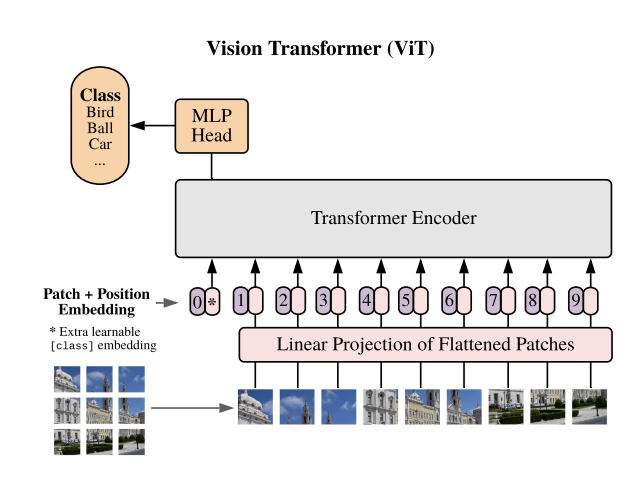
\includegraphics[width=0.8\textwidth]{fig/rel/images/vit_schema.png}
    \caption{\gls{vit} overview \autocite{dosovitskiy2020image}.}
    \label{fig:rel_vit}
\end{figure}
%--------------------------------------------------------------------------------------------------
\noindent In similar manner to prior breakthroughs like the effective convolution computation and the 
emergence of transformers in \gls{nlp}, the introduction of \gls{vit} further revolutionized the 
landscape on Computer Vision tasks. However, these methodologies exhibit specific characteristics 
concerning their predictive capabilities. In particular, when trained using a conventional 
approach for ImageNet object classification, the performance of this model is relatively low 
compared to a ResNet trained under the same conditions. However, when scaling to more modern 
datasets such as ImageNet-21k and JFT-300M \autocite{sun2017revisiting}, which contain close to 10 
times the number of images than those of ImageNet-1k, transformers clearly outperform their 
convolutional counterparts. Interestingly, this is hypothesized to be primarily due to transformer 
scalability. In particular, transformers are capable of removing inductive bias 
which in turn is highly dominant in \glspl{cnn}. Still, this makes these models prone to overfitting 
in data collections sufficiently small where this bias still remains useful.\\

%--------------------------------------------------------------------------------------------------
\noindent In addition to ViT, several other transformer architectures have emerged, contributing to 
the diversity and advancement of the field. One noteworthy example is PiT (Pooling in Transformer) 
\autocite{heo2021rethinking}, which re-introduces the concept pooling into transformers. To benefit 
from the hierarchical structure that is found in \glspl{cnn}, this operation is included with 
a modification for the pooling operation, where the image tokens are  pooled using depth-wise 
convolution. This inclusion of pooling is sustained by the measurement of \emph{attention entropy}, 
where this metric shows the spread and concentration of \emph{attention}; where in \gls{vit} this 
interaction is rather spread, and in PiT it is largely concentrated. Another significant 
development is Swin Transformer \autocite{liu2021swin}. Swin utilizes a shift-based windowing 
mechanism, allowing for efficient information processing across different scales. This design promotes 
enhanced modeling capabilities and facilitates the learning of intricate patterns in images.\\

%--------------------------------------------------------------------------------------------------
\noindent Indeed, since its proposal, \gls{vit} has dominated image recognition tasks. Still 
contrary the behavior \glspl{cnn} present as excellent feature extractors, ViTs underperform in 
areas such as image reconstruction and image reorganization. In particular, given the locality 
behavior and the inductive bias that these models present; these aforementioned tasks are 
consequently carried out in a better manner with CNNs. Nevertheless, similar to 
CNNs borrowing ideas from transformers as seen in \emph{ConvNeXt}; early stages in transformers 
dedicated to image patch encodings are replaced with convolutional layers, inheriting these 
characteristics for further downstream tasks. These models in turn are known as hybrid 
architectures.
%--------------------------------------------------------------------------------------------------
\subsection{Hybrid Architectures}
\label{rel:sub_hybrid}
Following the locality properties of \glspl{cnn} and globality of \glspl{vit}; it is proved 
that incorporating ideas from these architectures is feasible, generating a model that attends in 
to both local information and scales well with training data. In particular, some 
preliminary studies towards these combinations performed on ViT, suggested modifications of the 
architecture starting with the encoder. Starting with what is arguably the most basic \gls{cnn} 
design, LeViT \autocite{graham2021levit} replaces the original patch encoding with feature 
extraction using LeNet; as well as including a distillation head to lead the training process. 
These contributions ultimately helped LeViT to outperform ViT all the while not requiring large 
scale image classification datasets to train as well as having a faster inference time.\\

%--------------------------------------------------------------------------------------------------
\noindent As a continuation of LeViT, PatchConvNet \autocite{touvron2021augmenting} was subsequently 
proposed. Building upon the LeViT design, PatchConvNet further expands on the classifier by 
replacing the original MLP head with \emph{Attention-Based Pooling}. Interestingly, this 
pooling mechanism integrates a ([\Th{CLS}]) matrix; that in sharp comparison to the stand-alone 
token, is able to capture class-specific information. PatchConvNet ultimately improves  
recognition properties found in LeViT, while also showing promise in terms of segmentation and 
detection, suggesting that the model has built-in interpretability by the capability of 
visualizing the aforementioned class-specific attention. Nevertheless, the key contribution 
behind this architecture is derived from the convolutional stem, taken from LeViT.\\ 

%--------------------------------------------------------------------------------------------------
\noindent One key characteristic that \glspl{cnn} display is a certain degree of robustness 
regarding the optimizer choice during the training stage. This phenomenon was 
observed to be the opposite regarding \gls{vit}, the optimizer choice is crucial for these 
models. Similarly to LeViT, by the addition of early convolutions it is argued that 
this issue can be overcome, as proposed on \emph{Early convolutions help transformers see 
better} \autocite{xiao2021early}. Moreover, in this work a direct comparison between ViT trained 
using a patchifier, versus using convolutions; where \emph{Optimizability}\footnote{As defined by 
\cite{xiao2021early}, it refers to the presence of difficulties characterizing the training 
process of deep models while varying their optimizers, data augmentation and performance drop 
when scaling in size} is used to establish differences.\\

%--------------------------------------------------------------------------------------------------
\begin{figure}[t]
    \centering
    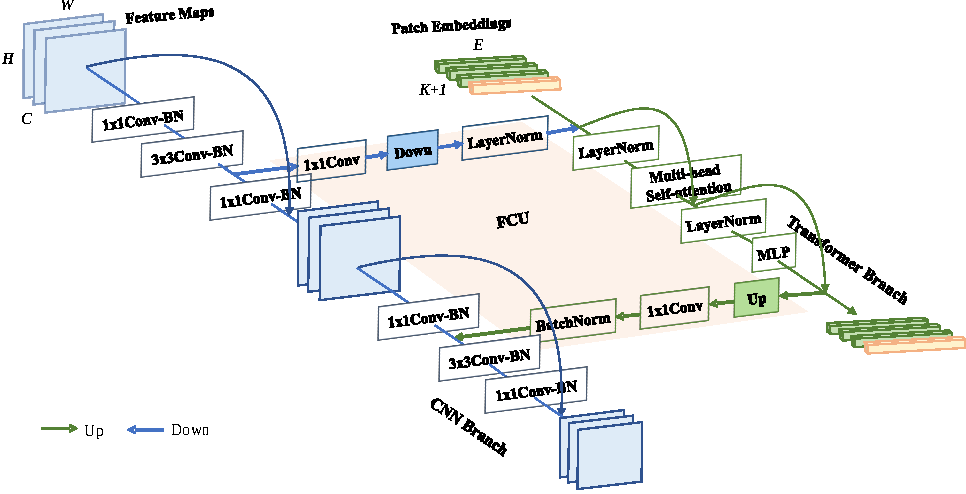
\includegraphics[width=0.8\textwidth]{fig/rel/images/conformer.pdf}
    \caption{\textbf{Conformer architecture} overview. \autocite{peng2021conformer}}
    \label{fig:rel_conformer}
\end{figure}
%--------------------------------------------------------------------------------------------------
\noindent In addition of including convolution atop \glspl{vit}, researchers have sought to propose 
ideas to combine the differences in processing between transformers and \glspl{cnn}. In an 
approach similar to Siamese networks, it is possible to interchange information and update 
features from one CNN to a transformer by implementing a coupling unit to lead this 
communication. One approach that encompasses this design idea is the \emph{Conformer} \autocite{
peng2021conformer}, where the \emph{Feature Coupling Unit} (FCU) is used to introduce information 
from a convolutional branch into a transformer one, and in the opposite direction as well. In 
particular, Conformer uses a ResNet architecture for its convolutional branch, while 
maintaining the first convolutions to process the image into image patches. For the transformer 
branch, this model introduces a modified ViT, where the number of encoder blocks is one element 
less than the totality of residual blocks. Moreover, the aforementioned FCU is introduced to update 
features in between residual blocks. Ultimately, any prediction is given by the average prediction 
between both branches. A detailed explanation of this model is found in \autoref{fig:rel_conformer}.